\mode<article>
{
  \usepackage{fullpage}
  \usepackage{pgf}
  \usepackage{hyperref}
  \usepackage{fancyvrb}
  \setjobnamebeamerversion{python.beamer}
}

\mode<presentation>
{
%  \usetheme{Szeged}
  %\usetheme{Dresden}
  \usetheme{Warsaw}
%  \usepackage{beamerthemebars}

  %\setbeamercovered{transparent}
}

\usepackage[T1]{fontenc}
\usepackage[utf8x]{inputenc}
%\usepackage{inputenc}
%\usepackage[magyar]{babel}
\usepackage{ucs}
\usepackage{tabularx}
\usepackage{fancyvrb}
\usepackage{booktabs}
%\usepackage[dvips]{graphicx}

%pygments-hez
\usepackage{fancyvrb}
\usepackage{color}
\input{style-defs}

\usepackage{tikz}
\usetikzlibrary{arrows}
\usetikzlibrary{patterns}
\usetikzlibrary{calc,backgrounds,positioning,fit}
\tikzset{ %inner sep = 0.5mm,
  %minimum size = 5mm,
  {selected path/.style} ={draw,opacity=.5,line width=3pt,green},
  {hide path/.style} ={selected path,white,opacity=.9},
  {base point/.style} ={circle,draw=blue!60,fill=blue!30,inner sep=0},
  {small point/.style} ={base point, minimum size= 1mm},
  {middle point/.style} ={base point, minimum size= 3mm},
  {large point/.style} ={base point, minimum size= 10mm},
  {future point/.style} ={circle,color=white,draw},
  point/.style ={circle,draw=black!60,fill=black!20},
  {new point/.style} ={point,fill=blue!30,draw=blue!60},
  {edge/.style} ={thick,draw},
  {new edge/.style} ={draw,thick,-, blue!50},
  {box/.style}={rectangle,  minimum height=1cm,
                anchor=south west, draw, rectangle,
                fill=yellow!20,text centered, text width= 4cm},
  >=latex,
  state/.style = {thick, circle, draw, color = black,
                  fill = red!20, minimum size = 6mm},
  finalstate/.style = {state, fill=green!20, double},
  automat/.style = {thick, draw, color = black, fill = #1!12,
                  minimum size = 10mm},
  automat/.default = black,
  point/.style ={circle,draw=blue!60,fill=blue!30,
                  inner sep=0, minimum size= 1mm},
 }

\author{Árpád Horváth}
\title{Data Visualization in Python}
%\subtitle{Informatika elméleti alapjai}
\subject{programming, python}
%\institute[ÓE AMK]{Óbudai Egyetem\\
%  Alba Regia Műszaki Kar (AMK)\\
%  Székesfehérvár}

% Delete this, if you do not want the table of contents to pop up at
% the beginning of each subsection:
\AtBeginSection[]
{
  \begin{frame}<beamer>
    {Vázlat}
    \tableofcontents[currentsection,currentsubsection]
  \end{frame}
}

\AtBeginSubsection[]
{
  \begin{frame}<beamer>
    {Vázlat}
    \tableofcontents[currentsection,currentsubsection]
  \end{frame}
}


\newlength{\maxheight}
\setlength{\maxheight}{0.63\textwidth}


\begin{document}

\frame{\maketitle}

% \begin{frame}
%   {Aktuális}
%   \begin{itemize}
%     \item <+-| alert@+> okt 18. --> okt 30. szerda 14:25 ZH
%     \item <+-| alert@+> django.amk.uni-obuda.hu:8888-on 01 02 és 03
%         kezdetű kell
%     \item <+-| alert@+> Python3-at használunk végig
%     \item <+-| alert@+> most már a django-n is az van
%     \item <+-| alert@+> első heti gyakorlatok print-jei
%     \item <+-| alert@+> itt (haladó) feliratú oldalak nem kellenek
%         IRA-hoz
%   \end{itemize}
% \end{frame}

\begin{frame}<beamer>
  {Vázlat}
  \tableofcontents
\end{frame}

%\tableofcontents


\section*{Introduction}

\begin{frame}[fragile]
    {Packages for Data Visualization}


\newlength{\basewidth}
\setlength{\basewidth}{10mm}

\begin{minipage}{.7\linewidth}
    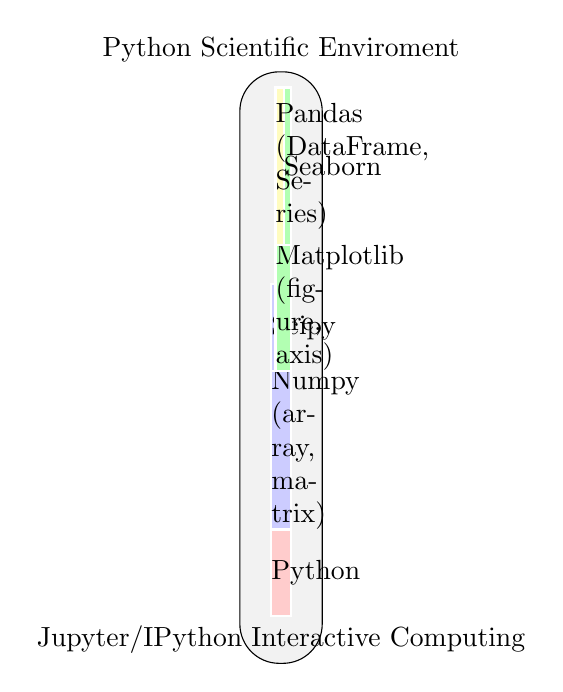
\begin{tikzpicture}[
	node distance = 0mm,
	block/.style args = {#1,#2}{fill=#1,
	text width=#2,
	shape=rectangle, draw=white, thick,
	minimum height=11mm, align=center,
	inner sep=0mm, outer sep=0mm}
	]
	\node[block={red!20,7\basewidth},
	label=below:Jupyter/IPython Interactive Computing]
	(python)    {Python};
	\node[block={blue!20,7\basewidth},
	above right=of python.north west] (numpy) {Numpy (array, matrix)};
	\node[block={blue!20,1.5\basewidth},
	above right=of numpy.north west]  (scipy) {Scipy};
	\path   let \p1 = (numpy.south west),
	\p2 = (scipy.north west),
	\n1 = {veclen(\x2-\x1,\y2-\y1)} in
	node[block={green!30,5.5\basewidth},minimum height=11mm,
	above left=of numpy.north east]
	(matplotlib) {Matplotlib (figure, axis)}
	node[block={green!30,2.5\basewidth},minimum height=20mm,
	above left=of matplotlib.north east]
	(seaborn) {Seaborn}
	;
	\node[block={yellow!25,3.0\basewidth},minimum height=20mm,
	left=of seaborn]        (pandas)    {Pandas (DataFrame, Series)};
	\scoped[on background layer]
	\node[rounded corners=5mm,fill=gray!10, draw,
	inner sep=4mm,yshift=-2mm,
	label=above:Python Scientific Enviroment,
	fit=(python) (seaborn)]  {};
    \end{tikzpicture}
\end{minipage}
\begin{minipage}{.27\linewidth}
    \begin{itemize}
	\item Pylab = Numpy + Matplotlib\\
	     $\approx$ MATLAB
	\item Web-centric Visualisation Libraries:
	    bokeh, plotly
    \end{itemize}
\end{minipage}
\end{frame}

\section{Initial settings and imports}

\begin{frame}
    {Jupyter notebook vs script}

    Jupyter notebook
    \begin{itemize}
        \item We need a web browser.
        \item Set a password (bash commands).
        \item Easy to run the parts several times with small modifications.
        \item Titles and texts can be added easily (LaTeX equations as well).
        \item Easy to share (as is, as HTML, PDF\ldots).
        \item We can restart the kernel and run all the cells.
    \end{itemize}

    Script
    \begin{itemize}
        \item Easy to structure (modules, packages).
        \item Doesn't need Jupyter to install.
        \item IDE-s with more capabilities (version control, renaming).
    \end{itemize}
\end{frame}

\begin{frame}[fragile]
    {ms.version}

    % TODO
\end{frame}


\begin{frame}[fragile]
    {Imports used here}


\input{codes/visualization/pandas_numpy_imports.py.listing}

In interactive sessions, instead of the first two lines:

\begin{Verbatim}
from pylab import *
\end{Verbatim}

Do not use in scripts!
\end{frame}


\section{Examples}
\subsection{Matplotlib}

\begin{frame}[fragile]
  {First plots with matplotlib}

\scriptsize
\input{codes/visualization/first_plot.py.listing}

No needs of \verb+np.+ and \verb+plt.+ with \verb+from pylab import *+ or
\begin{Verbatim}
from numpy import linspace, pi
from matplotlib.pyplot import (plot, legend, savefig,
           close, xlabel, ylabel, title, grid)
\end{Verbatim}
\end{frame}

\begin{frame}
    {The results}

 \includegraphics[width=.48\textwidth]{codes/visualization/first.pdf}
 \includegraphics[width=.48\textwidth]{codes/visualization/trigonometry.pdf}
\end{frame}

\begin{frame}
  {Bar plots and colors, tight layout}

\scriptsize
\input{codes/visualization/bar_plots.py.listing}

  \includegraphics[width=.7\textwidth]{codes/visualization/bar_plots.pdf}
\end{frame}

\subsection{Pandas and Seaborn}

\subsection{Further reading}



\section*{Conclusion}
\addcontentsline{toc}{section}{Conclusion}

\end{document}

\begin{frame}
    {Packages for Data Visualization}

\newcommand{\basewidth}{1.2 cm}
\begin{tikzpicture}[x=\basewidth, y=1cm, node distance=0 cm,outer sep = 0pt]
% Style for Days
\tikzstyle{text field}=[rectangle,  minimum height=1cm,
  anchor=south west]
\tikzstyle{box}=[text field, draw, rectangle,
  fill=yellow!20,text centered, text width= 1cm]

\tikzstyle{1units}=[box,minimum width=1.2 cm, text width=1cm]
\tikzstyle{2units}=[box,minimum width=2.4 cm, text width=2.2cm]
\tikzstyle{3units}=[box,minimum width=3.6 cm, text width=3.4cm]
\tikzstyle{5units}=[box,minimum width=6 cm  , text width=5.8cm]
%Style for type of sequence 
% Positioning labels for days and hours
\node[3units,fill=yellow!30] at (0,0) {libigraph (C)};
\node[3units,fill=yellow!30] at (0,1) {IGraph (Python)};
\node[2units] at (3,0) {numpy};
\node[2units] at (3,1) {matplotlib/ pylab};
%\node[2units] at (5,0) {\color{black!70} readlines};
%\node[2units] at (5,1) {\color{black!70} ipython};
\node[5units,fill=red!30] at (2,2) {cxnet};
\node[2units,fill=red!20] at (0,2) {mfng};
\draw[fill=blue!20] (1.5,3) -- (1.5,5) -- (2,5) -- (2,3);
\draw[fill=blue!20] (0,3) -- (7,3) -- (3.5,5) -- cycle;
\node[text centered, text width=3.6cm] at (3.5,3.7) {documentation,
educational material};

\tikzstyle{rotated text field}=[text field, minimum height=\basewidth,
  minimum width=2cm, rotate=90, fill=yellow!20]
\node[rotated text field,draw] at (6,0) {\color{black!70} \small python-apt};
\node[rotated text field,draw] at (7,0) {\color{black!50} ipython};
\end{tikzpicture}
\end{frame}

\begin{frame}
  {Mi a Python?}
  \begin{itemize}
    \item <+-| alert@+> Általános célú programnyelv
    \item <+-| alert@+> rengeteg beépített és egyéb modullal.
\includegraphics[width=0.7\textwidth]{img/Python_batteries_included.jpg}
    \item <+-| alert@+> Dinamikusan típusos (egyszer egész másszor
        lista)
    \item <+-| alert@+> Objektumorientált (adattípusoknak saját
        függvényei lehetnek)
    \item <+-| alert@+> Platformfüggetlen bytekódot készít
    \item <+-| alert@+> Könnyen beágyazhatóak C és Fortran programok
        (Pylab)
  \end{itemize}
\end{frame}

\begin{frame}
  {Példaprogram -- feladatkitűzés}
  Készítsünk egy függvényt, amely a
  \[ax^2+bx+c=0\]
  egyenlet gyökeit adja vissza.

  A gyökök:
  \[x_{1,2}= \frac {-b \pm \sqrt{b^2 - 4ac}} {2a}\]
\end{frame}

\begin{frame}
  {Példaprogram -- megvalósítás}
  \small
  \input{codes/masodfoku.py.listing}
\end{frame}

\begin{frame}
  {A szerző}
  \begin{columns}[t, onlytextwidth]
   \column[T]{0.49\textwidth}
  \begin{itemize}
    \item <+-| alert@+> Guido von Rossum, holland
    %\item <+-| alert@+> BDFL -- Benevolent Dictator for Life
    \item <+-| alert@+> Jelenleg a Dropbox, korábban a Google alkalmazottja
  \end{itemize}
   \column[T]{0.49\textwidth}
  \only<1>{\includegraphics[width=0.7\textwidth]{img/Guido_van_Rossum_OSCON_2006.jpg}}
  \only<2>{\includegraphics[width=\textwidth]{img/who_is_guido_keretes.jpg}}
  \end{columns}
\end{frame}

\begin{frame}
  {Miért Python?}
  \begin{columns}[t, onlytextwidth]
   \column[T]{0.59\textwidth}
  \begin{itemize}
    \item <1-| alert@1> Na vajon miért?
    \item <2-| alert@2> A szerző kedvence a Monty Python's Flying Circus
    \item <3-| alert@3> A dokumentációban ajánlott a Monty Python idézet
  \end{itemize}
   \column[T]{0.39\textwidth}
  \only<1>{\includegraphics[width=\textwidth]{img/python.jpg}}
  \only<2>{\includegraphics[width=\textwidth]{img/monty_python_and_the_holy_grail.jpg}}
  \only<3>{\includegraphics[width=\textwidth]{img/monty-python.jpeg}}
  \end{columns}
\end{frame}

\subsection[Adatszerkezetek]{A Python adatszerkezetei}
\begin{frame}[fragile]
  {Számok }
  \begin{itemize}
    \item <+-| alert@+> egész (int)
\\\verb!1, 2123123123123123118978970!
    \item <+-| alert@+> lebegőpontos (float)
\\\verb!3.14, 1.6e-19!\\ (math modul)
    \item <+-| alert@+> komplex (complex)
\\\verb!1+3j, 2j!\\ (cmath modul)
    \item <+-| alert@+> Műveletek +, -, *, /, ** (hatvány)
    \item <+-| alert@+> Műveletek egészeknél \% (mod), //,
        bitenkénti műveletek\\
  \end{itemize}
\end{frame}

\begin{frame}[fragile]
  {Karakterláncok (str, sztring)}
  \begin{itemize}
    \item <+-| alert@+> \verb!'Szelet', 'alma\nkörte', "that's it"!
    \item <+-| alert@+> Többsoros karakterlánc
\begin{Verbatim}[frame=single]
'''A többsoros szövegeket
három idézőjel (" vagy ')
határolja.'''
\end{Verbatim}
    \item <+-| alert@+> Metódusok: split, splitlines, upper, center,
        rjust, format\dots
    \item <+-| alert@+>  Műveletek: +
    \item <+-| alert@+>  \verb!'AMK '*3  # AMK AMK AMK!
  \end{itemize}
\end{frame}

\begin{frame}[fragile]
  {Karakterláncok format metódusa (haladó)}

  \input{codes/format.py.listing}
\end{frame}

\begin{frame}[fragile]
  { Listák (list)}
  \begin{itemize}
    \item <+-| alert@+> Bármilyen típusú elemei lehetnek\\
   \verb!l = [1, 'alma', 2+3j, [5, 4]]!
    \item <+-> \alert{Módosíthatjuk}: hozzáfűzhetünk,
beszúrhatunk és törölhetünk belőle elemeket
    \item <+-| alert@+> Metódusai: append, insert, count, pop\dots
    \item <+-> Példák:
   \input{codes/lista.py.listing}
  \end{itemize}
\end{frame}

\begin{frame}[fragile]
  { Rendezett sorozatok (tuple)}
  \begin{itemize}
    \item <+-> Listához hasonló, de \alert{nem módosítható}
    \item <+-| alert@+> \verb!t = (1, 'AREK', [1,2])!
    \item <+-> Példák értékadásra:
   \input{codes/tuple.py.listing}
  \end{itemize}
\end{frame}

\begin{frame}[fragile]
  {Sorozattípusok közös jellemzői}
  \begin{itemize}
    \item <+-| alert@+> Sorozattípusok: karakterlánc, lista,
        tuple\ldots
    \item <+-| alert@+> Ezeknél működik az indexelés és szeletelés.
    \item <+-| alert@+> 0. elemmel kezdünk. (ahogy C-ben, de MATLAB-ban
        1-től)
    \item <+-| alert@+> \verb!s = 'Szelet'! \\
% \small
% \begin{verbatim}
%  +---+---+---+---+---+---+
%  | S | z | e | l | e | t |
%  +---+---+---+---+---+---+
%    0   1   2   3   4   5   6
%   -6  -5  -4  -3  -2  -1
% \end{verbatim}
    \item <+-| alert@+> Példák:\\
        \hspace{-3em}
	\verb!s[0], s[2:4], s[:3] = s[0:3], s[-2:] = s[-2:6], s[2:-2]!
    \item <+-| alert@+> A felső határ nincs bent sohasem: 2:5 = 2, 3, 4.
    \item <+-| alert@+> Használható a \verb!len()! (hossz) függvény
        rájuk. \verb!len('Szelet') == 6!
    \item <+-| alert@+> Használható a \verb!max()! és \verb!min()!
	függvény rájuk, számoknál \verb!sum()!
    \item <+-| alert@+> Benne van-e elem: \verb!1 in (1,4,2) # True!
  \end{itemize}
\end{frame}

\begin{frame}[fragile]
    {Függvények és hívásuk}

    Függvények jellemzői:
    \begin{itemize}
        \item argumentumaik lehetnek (zárójelben felsorolva, vesszővel
            elválasztva)
        \item csinálhatnak valamit (print kiír képernyőre)
        \item visszatérnek valamilyen értékkel (esetleg \verb!None!-nal)
    \end{itemize}

    Függvények hívása:
    \begin{itemize}
        \item kulcsszavas argumentumok (többi után)\\
            \verb!print(1, 3, 'alma', sep=':', end='\n\n')!
        \item alapértelmezett értékek (\verb!sep=' ', end='\n'!), ha nem adom meg, azt
            használja
    \end{itemize}
\end{frame}

\begin{frame}[fragile]
  { Szótárak (dict) (haladó)}
  \begin{itemize}
    \item <+-| alert@+> Egy kulcs azonosít egy elemet.
    \item <+-> Példák:
   \input{codes/dictionary.py.listing}
    \item <+-> Csak \alert{nem-módosítható elem} lehet kulcs.
  \end{itemize}
\end{frame}

\begin{frame}[fragile]
  {Logikai (bool)}
  \begin{itemize}
    \item <+-| alert@+> Értéke lehet True és False.
    \item <+-| alert@+> Vizsgálatnál hamis értékűek (a nullák és az ,,üresek''):\\
	\verb!0   0.0  0+0j   []   ()   ''   {}!
    \item <+-> Példák:
   \input{codes/boolean.py.listing}
  \end{itemize}
\end{frame}

\begin{frame}
    {Adattípusok egymásba alakítása}

    \input{codes/convert.py.listing}
\end{frame}

\begin{frame}
    {Adattípusok összefoglalása}

    \begin{tabular}{rl}
	\toprule
	megváltoztatható (mutable)& nem az (immutable)\\
	\midrule
	&int,float,complex\\
	&str\\
	list&tuple\\
	set&frozenset\\
	dict&\\
	&bool\\
	\bottomrule
    \end{tabular}

    A jobboldaliak lehetnek szótárak indexei.
\end{frame}

\subsection[Vezérlési szerkezetek]{A Python vezérlési szerkezetei}

\begin{frame}[fragile]
  {A Python vezérlési szerkezetei}
  \begin{itemize}
    \item <+-| alert@+> \verb!if while for def class try!
    \item <+-| alert@+> Vázlatosan:
\begin{Verbatim}[frame=single]
szerkezet eleje:
    első utasítás
    második utasítás
    harmadik utasítás
ez már nincs benne
\end{Verbatim}
    \item <+-| alert@+> Fontos a \verb!:! és a behúzások.
  \end{itemize}
\end{frame}

\begin{frame}[fragile]
  {Feltételes elágazás Pythonban}
      \input{codes/if.py.listing}
\end{frame}

\begin{frame}[fragile]
  {Függvények Pythonban}
  \small
      \input{codes/masodfoku.py.listing}
\end{frame}

% \begin{frame}[fragile]
%   {Komplex változat (haladó)}
%   \small
%       \input{codes/cmasodfoku.py.listing}
% \end{frame}

\begin{frame}[fragile]
  {for ciklus Pythonban}
  \begin{itemize}
    \item <+-| alert@+> Python példa; fontos a \verb!:! és a behúzások:
\begin{Verbatim}[frame=single]
szoveg = 'alma'
for karakter in szoveg:
    print karakter
    print karakter.upper()
\end{Verbatim}
    \item <+-| alert@+> Általános alakja:
\begin{Verbatim}[frame=single]
for <változó> in <sorozat>:
    <parancsok egyformán behúzva>

<parancs, ami már nincs a ciklusban>
\end{Verbatim}
    \item <+-| alert@+> A sorozat lehet például lista vagy tuple, ekkor az
elemeiken megy végig a ciklus, de lehet karakterlánc is, akkor a
karakterein.
  \end{itemize}
\end{frame}

\begin{frame}[fragile]
  {for ciklus Pythonban -- range}
  \begin{itemize}
    \item <+-| alert@+> Gyakran használjuk for-ral a \verb!range(n)! függvényt.
    \item <+-| alert@+-> \verb!range([start,] stop[, step])!
    \item <+-| alert@+-> Listává alakítva:
    \item <+-| alert@+> \verb!range(5) ==> [0, 1, 2, 3, 4]!
    \item <+-| alert@+> \verb!range(2, 5) ==> [2, 3, 4]!
    \item <+-| alert@+> \verb!range(2, 8, 3) ==> [2, 5]!
  \end{itemize}
\end{frame}

\begin{frame}[fragile]
  {Ciklus és számtípusok}
\begin{Verbatim}[label=példa, frame=single]
for i in [1, 1.03, 1j, 5]:
    print i, i**100

Eredmény:
    1 1
 1.03 19.2186319809
   1j (1+0j)
    5 7888609052210118054117285652827862296732064351090230047702789306640625
\end{Verbatim}
\end{frame}

\begin{frame}
    [fragile]{Listaértelmezés (szótár-, halmazértelmezés)}

      \input{codes/list_comp.py.listing}
\end{frame}

\begin{frame}[fragile]
  {while ciklus Pythonban}
      \input{codes/Euklidesz.py.listing}
\end{frame}

\begin{frame}[fragile]
  {while ciklus Pythonban}
    Eredmény:
\begin{Verbatim}
 2850  2310
 2310   540
  540   150
  150    90
   90    60
   60    30
A legnagyobb közös osztó: 30
\end{Verbatim}

%     \item <+-| alert@+>  Lehet máshogy cserélni:
% \begin{Verbatim}
% a, b = (a,b)  if a>b else (b,a)
% # C-ben: feltétel?igaz-érték:hamis-érték
% \end{Verbatim}
\end{frame}

\begin{frame}[fragile]
{Python 3-as verzió}

\begin{itemize}
    \item Nem teljesen kompatibilis a 2-essel. Pár elavult dolgot helyreraktak.

    \item Függvény lett a print: print(1, 'alma', sep=':', file=f)

    \item range nem hoz létre listát.
        for-ban ugyanúgy használható, ha lista kell
        list(range(10000))

    \item Külső modulok nem mind léteznek még 3-ashoz.

    \item Alapból utf-8 kódolás (nem kell megadni). Ékezetes sztringek könnyebb kezelése.

    \item Általában python3 utasítással indíthatjuk, ha telepítve van.

    \item Pár dolog python2 újabb változataiban is használható:
\begin{Verbatim}[commandchars=\\\{\}]
    \PY{k+kn}{from} __future__ \PY{k+kn}{import} \PY{n}{division} \PY{c}{\PYZsh{} 1/2 = 0.5}
    \PY{k+kn}{from} __future__ \PY{k+kn}{import} \PY{n}{print_function}
\end{Verbatim}
\end{itemize}
\end{frame}

\section{A Python moduljai}
\subsection{Modulok kezelése}
\begin{frame}[fragile]
  {Saját modulok (haladó)}
      \input{codes/modul.py.listing}
      \vfill

      Hogyan használhatom modulként? Mi fut le importáláskor?

      \vfill
      Figyeljük meg, hány aláhúzás van?
\end{frame}

\begin{frame}[fragile]
  {Saját modulok (haladó)}
      \input{codes/modul.py.listing}
	\vfill
      \input{codes/modulhivo.py.listing}
\end{frame}

\begin{frame}[fragile]
  {Almodulok}
  \begin{itemize}
    \item <+-| alert@+> A modulok gyakran almodulokat is
tartalmazhatnak.
    \item <+-| alert@+> Például az os modul path almoduljában vannak az
útvonalak összerakásával, szétszedésével kapcsolatos függvények.
    \item <+-> Példák:
\begin{semiverbatim}
\alert<3>{import os
os.path.join('python', 'nx', 'xx.py')}
\alert<4>{python/nx/xx.py (Un*x),} \alert<5>{python\textbackslash{}nx\textbackslash{}xx.py (Windows)}

\alert<6>{from os import path
path.join('python', 'nx', 'xx.py')}

\alert<7>{from os.path import join}
\alert<8>{from os.path import *}
\alert<7-8>{join('python', 'nx', 'xx.py')}
\end{semiverbatim}
  \end{itemize}
\end{frame}

\subsection{Példák modulokra}
\begin{frame}
  {Standard könyvtár}
  \begin{itemize}
    \item Bővebben http://docs.python.org \alert{The Python Standard
            Library}
    \item os: az operációs rendszerrel kapcsolatos
dolgokban segít (fájlmásolás, link létrehozása, parancs végrehajtása)
    \item sys: a Python működésével kapcsolatos
modul (elérési útvonal, argumentumok kezelése)
    \item urllib: a weboldalak eléréséhez.
    \item re: reguláris kifejezések kezeléséhez
    \item random: véletlen számok (egyenletes vagy normáis
eloszlású véletlen szám, visszatevés nélküli mintavétel listából)
    \item subprocess: alfolyamatok kezelése
    \item xml: XML-el kapcsolatos modul
    \item cgi, cgitb: CGI-szkripteléssel kapcsolatos modulok
    \item gettext: programok embernyelvi fordításához (en, hu, de)
    \item unittest, doctest: programok teszteléséhez
  \end{itemize}
\end{frame}

\begin{frame}
  {Külső modulok}
  \begin{itemize}
    \item  numpy: mátrixműveletek, lineáris egyenletek
    \item  pylab ($\in$ matplotlib): a MATLAB-hoz hasonló stílusú
        számítások, függvényrajzolás, numpy-t használja
    \item  scipy: szélsőértékkezelés, numerikus integrálás, \ldots
    \item  sympy: szimbolikus egyszerűsítés, differenciálás, integrálás
	(live.sympy.org)
    \item  NetworkX: gráfok kezelése, kirajzolása matplotlibbel
    \item  igraph: gráfok kezelése és kirajzolása, gyors,
        kirajzoláshoz nem kell matplotlib
    % \item cxnet: az igraphra épülő gráfelemző
    \item  flask, django: web-keretrendszer
    \item  PIL és Pillow: Python Image Library és utóda, képek feldolgozása,
        adataik kinyerése
    \item pandas: adatanalízis
    % \item  PyTables: nagy mennyiségű hierarchikus adat kezelése
    % \item  Star-P: A numpy párhuzamos rendszerekre írt
  \end{itemize}
\end{frame}

\begin{frame}[fragile]
  {Pylab}
      \input{codes/fourierpy_rovid.py.listing}
\end{frame}

\begin{frame}[fragile]
  {Adatbázis: DB API 2.0 (haladó)}
      \input{codes/database.py.listing}
\end{frame}

\begin{frame}[fragile]
  {CGI (haladó)}
      \input{codes/cgi.py.listing}
\end{frame}

\begin{frame}
  {flask / django}

  Az SQL-utasításokat és a CGI-t kiválthatjuk a django
  web-keretrendszerrel, vagy az \alert{SQLAlchemy}-vel, amit használhatunk pl. a
  flask mikro-webkeretrendszerrel.

  http://djangoproject.com
\end{frame}

\begin{frame}
    {Django}

    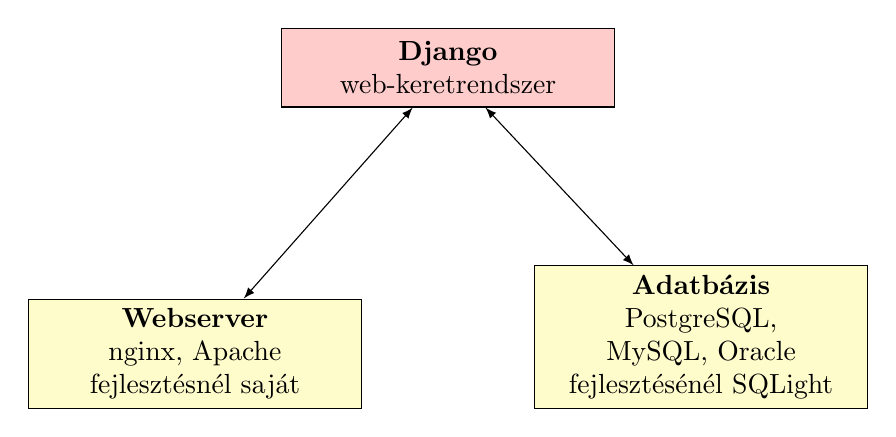
\begin{tikzpicture}[>=latex]
	\node[box,fill=red!20] (nyelv) at (0,0) {\textbf{Django}\\
	web-keretrendszer};
	\node[box] (nyelvtan) at (230:5) {\textbf{Webserver}\\nginx, Apache\\fejlesztésnél saját};
        \node[box] (automata) at (310:5)
	{\textbf{Adatbázis}\\PostgreSQL, MySQL, Oracle\\fejlesztésénél SQLight};
        \draw[<->] (nyelvtan) -- (nyelv);
        \draw[<->] (automata) -- (nyelv);
    \end{tikzpicture}
\end{frame}

\begin{frame}
    {Továbbiak}

    \begin{itemize}
	\item kulcsszavas argumentumok
	\item osztályok
    \end{itemize}
\end{frame}

%%%%%%%%% Vigyázz! Vége következik. %%%%%%%%%%
\end{document}
